\documentclass[12pt, twoside]{article}
\usepackage[francais]{babel}
\usepackage[T1]{fontenc}
\usepackage[latin1]{inputenc}
\usepackage[left=7mm, right=7mm, top=7mm, bottom=7mm]{geometry}
\usepackage{float}
\usepackage{graphicx}
\usepackage{array}
\usepackage{multirow}
\usepackage{amsmath,amssymb,mathrsfs}
\usepackage{soul}
\usepackage{textcomp}
\usepackage{eurosym}
 \usepackage{variations}
\usepackage{tabvar}

\begin{document}


\section*{\center{Aide individualis�e: Equations de droites}}

\subsection*{Exercice 1}

\textit{Passez directement � la question b).}

\medskip

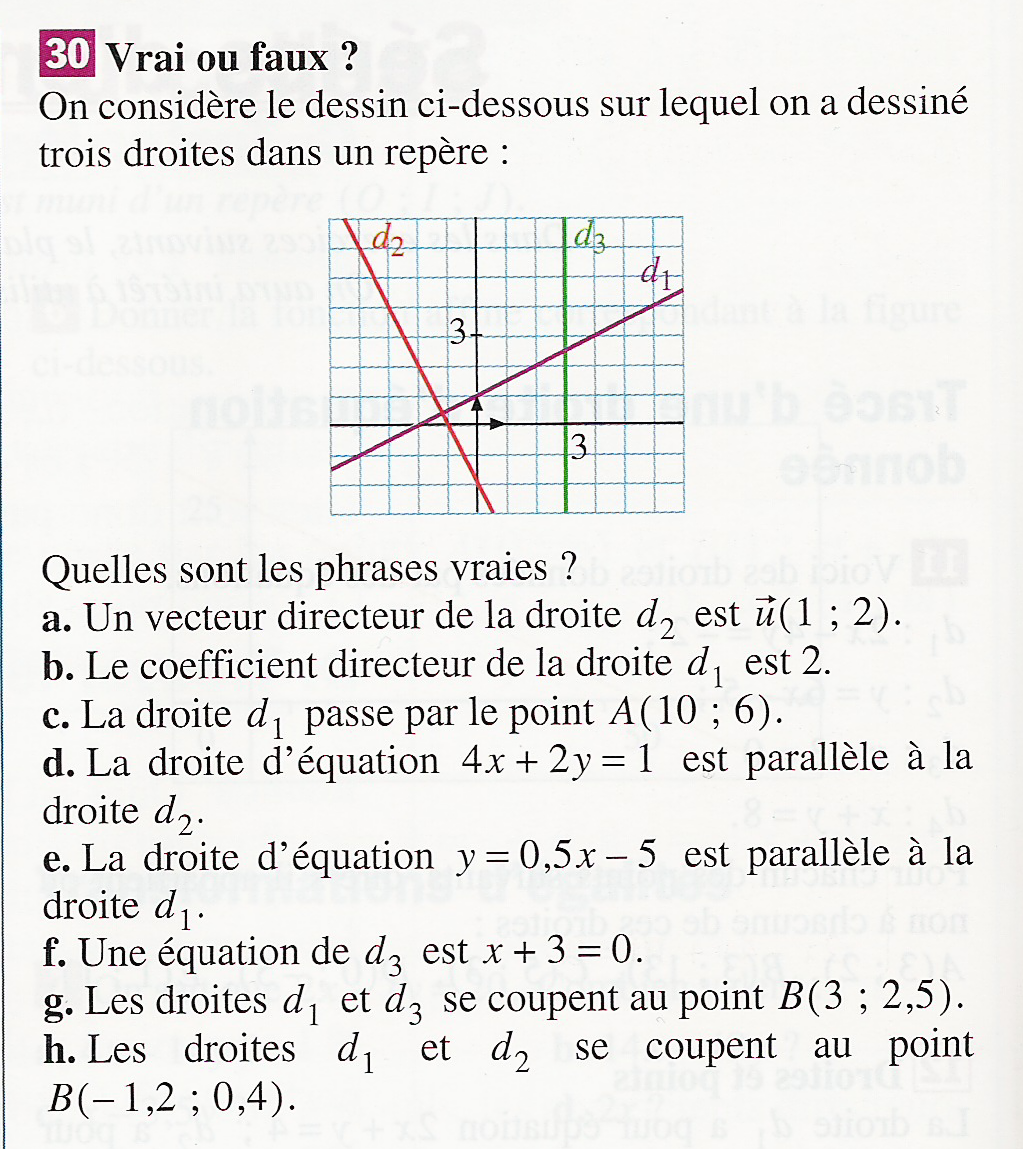
\includegraphics[width=9cm]{images/image1.png}


\subsection*{Exercice 2}

D�terminer les �quations des droites repr�sent�es ci-dessous. 
Pour cela, vous pouvez compl�ter le tableau \textbf{lorsque cela est possible}.

\medskip

\begin{tabular}{cc}
\begin{minipage}{9cm}
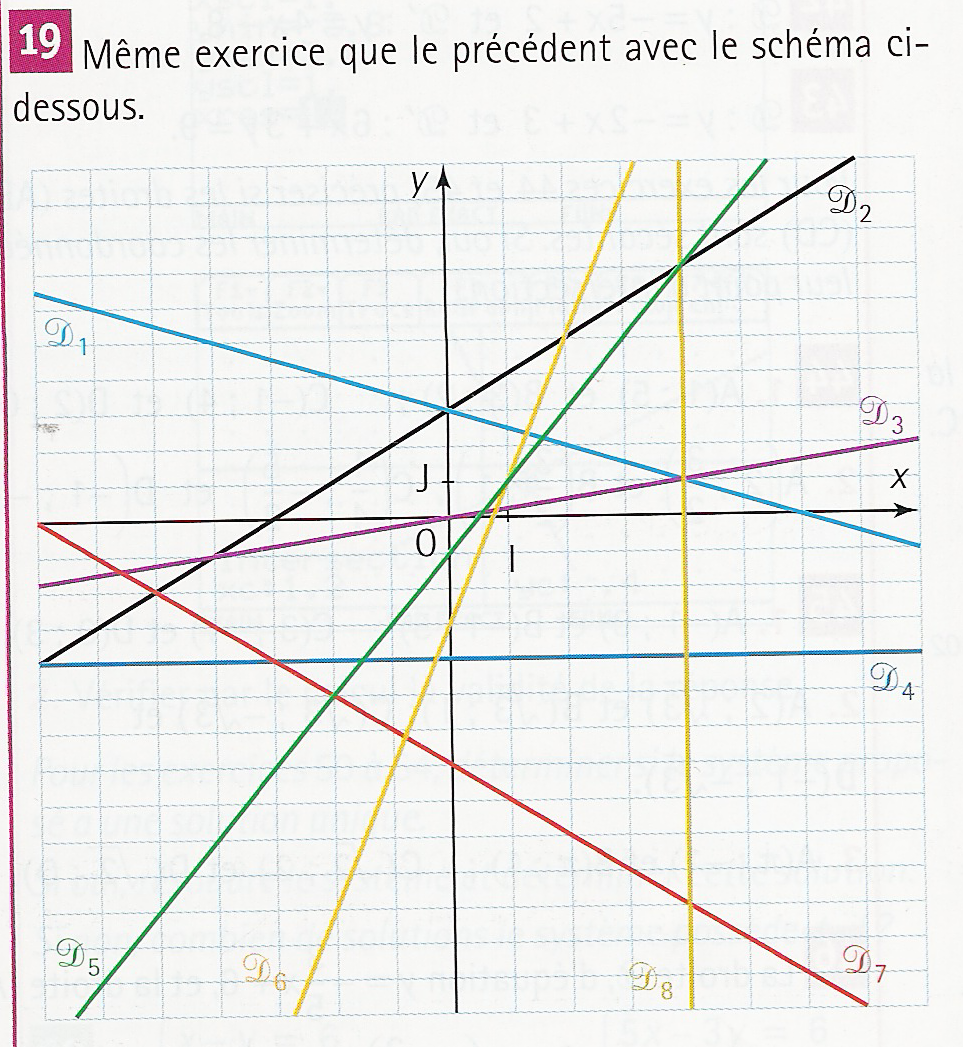
\includegraphics[width=9cm]{images/image2.png}
\end{minipage}
&
\begin{minipage}{9cm}
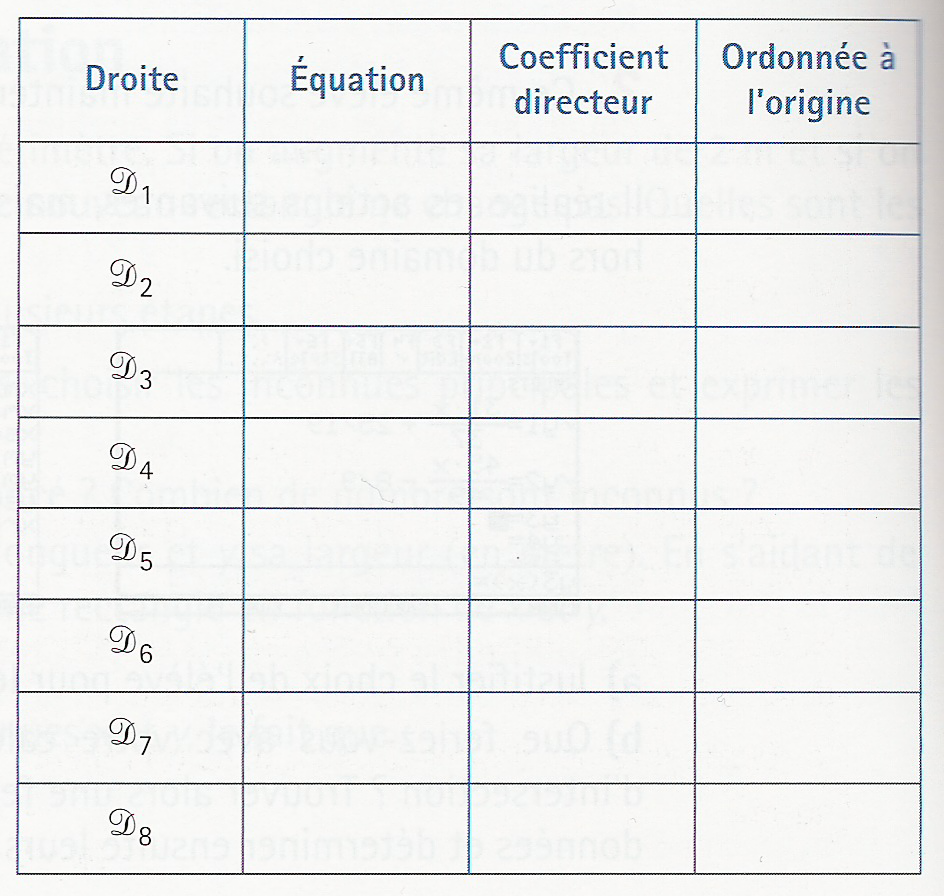
\includegraphics[width=9cm]{images/image3.png}
\end{minipage}
\end{tabular}


\end{document}
